%---------------------------------------------------------
%	4. MODELING & EVALUATION (numbers: DarkIR paper, arXiv 2412.13443)
%---------------------------------------------------------
\section{Results}

\begin{frame}
    \frametitle{Model Experimentation}
    \framesubtitle{Baselines vs.\ advanced models on LOLBlur}

    \begin{columns}[t]
        \begin{column}{0.56\textwidth}
            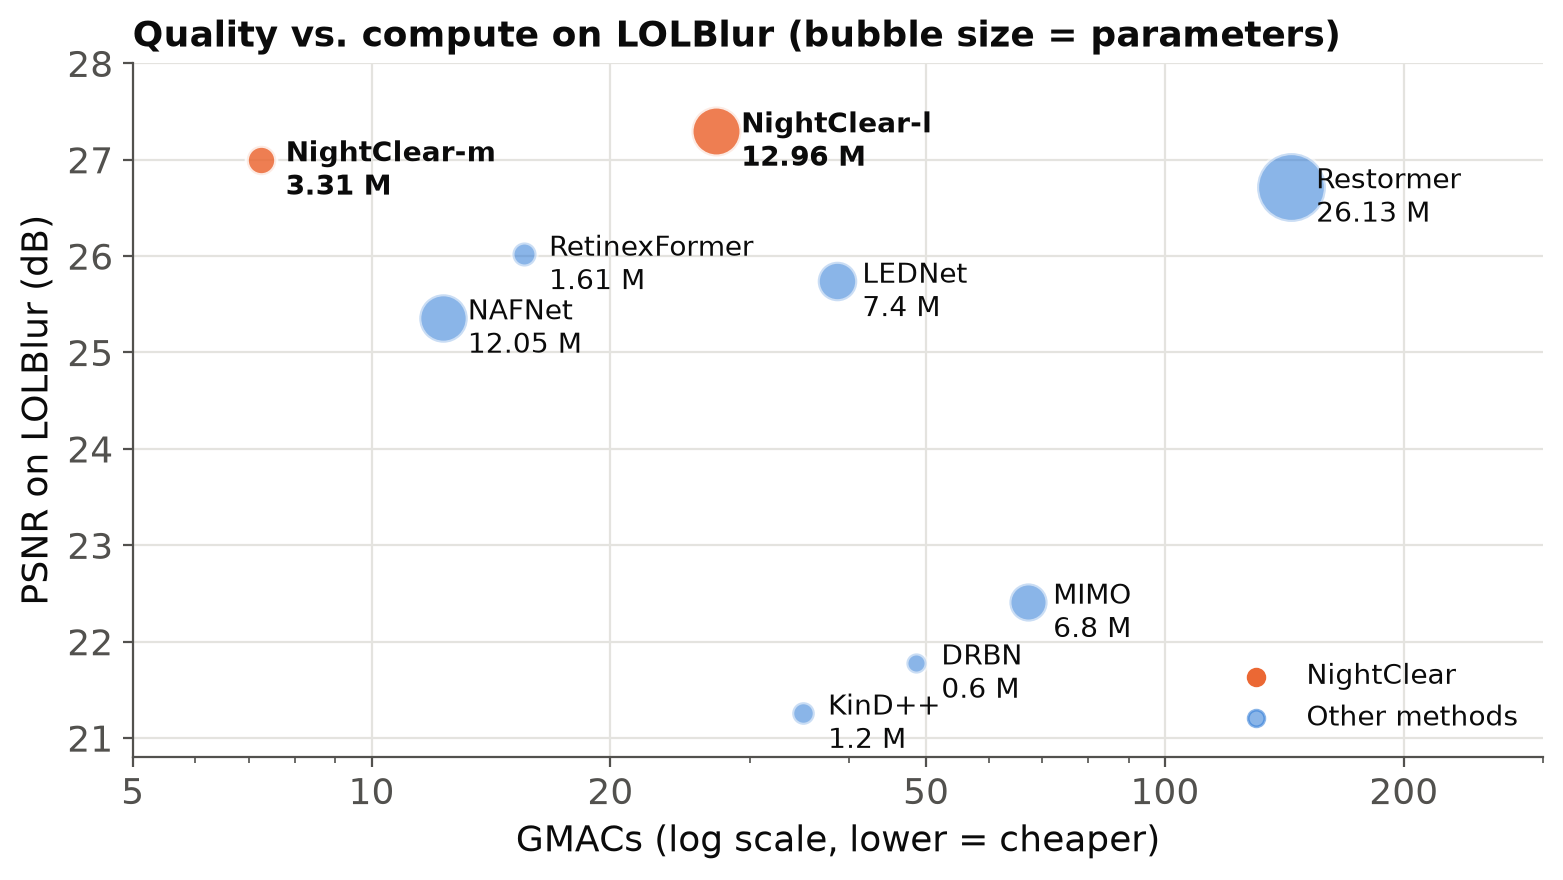
\includegraphics[width=\textwidth, height=0.55\textheight, keepaspectratio]{results/efficiency.png}\\
            \footnotesize NightClear-m reaches the best PSNR with the \textbf{lowest compute} (7.25 GMACs, 20$\times$ less than Restormer).
        \end{column}
        \begin{column}{0.42\textwidth}
            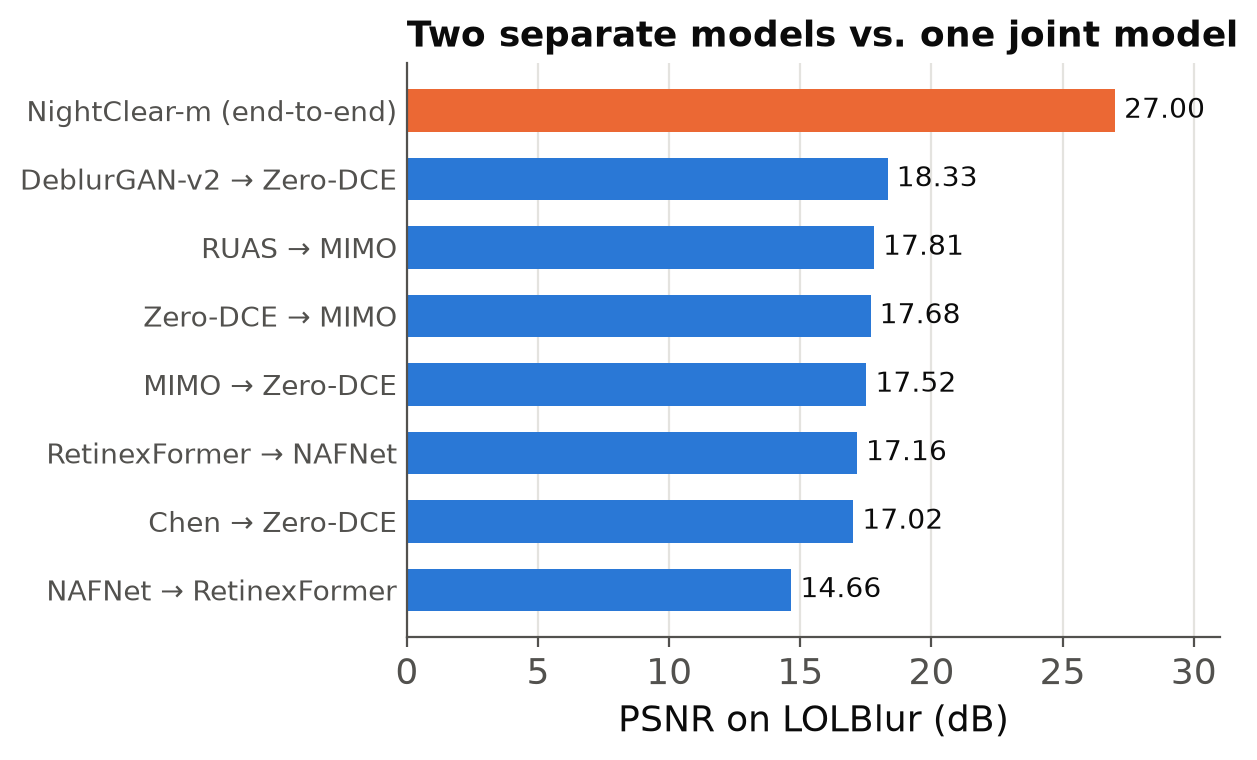
\includegraphics[width=\textwidth, height=0.55\textheight, keepaspectratio]{results/cascade.png}\\
            \footnotesize Every two-model cascade stays below 18.4\,dB; one joint model gains \textbf{+8.7\,dB}.
        \end{column}
    \end{columns}
    \vspace{1mm}
    {\tiny DeblurGAN-v2 (22.30 dB) is not plotted: no MACs available.}
\end{frame}

\begin{frame}
    \frametitle{Evaluation Across Datasets}
    \framesubtitle{Best other method per row; bold = better value}

    \begin{center}
    \footnotesize
    \begin{tabular}{lllll}
        \toprule
        \textbf{Dataset} & \textbf{Metric} & \textbf{NightClear} & \textbf{Best other method} & \\
        \midrule
        LOLBlur & PSNR $\uparrow$  & \textbf{27.00} (m) / \textbf{27.30} (l) & 26.72 & Restormer \\
                & SSIM $\uparrow$  & 0.883 / 0.898 & \textbf{0.902} & Restormer \\
                & LPIPS $\downarrow$ & 0.162 / 0.137 & \textbf{0.133} & Restormer \\
        LOLv2-real  & PSNR / SSIM & \textbf{23.87} / \textbf{0.880} & 22.80 / 0.840 & Retinexformer \\
        LOLv2-synth & PSNR / SSIM & 25.54 / \textbf{0.934} & \textbf{25.67} / 0.930 & Retinexformer \\
        LSRW        & PSNR / SSIM & \textbf{18.93} / \textbf{0.583} & 17.67 / 0.549 & FIDE \\
        Real-LOLBlur & MUSIQ $\uparrow$ / NIQE $\downarrow$ & 48.36 / 4.998 & \textbf{50.22} / \textbf{4.576} & NAFNet / Retinexformer \\
        \bottomrule
    \end{tabular}
    \end{center}
    \vspace{1mm}
    \footnotesize
    \begin{itemize}
        \item Best PSNR on 3 of the 4 paired benchmarks, with 8$\times$ fewer parameters than Restormer.
        \item Not the best everywhere: Restormer has better SSIM / LPIPS on LOLBlur, and on real blurry night photos (no GT) NightClear is competitive but not first.
    \end{itemize}
    {\tiny LOLv2 / LSRW use NightClear-mt (multi-task model, 26.62 dB on LOLBlur).}
\end{frame}

\begin{frame}
    \frametitle{Error Analysis}
    \framesubtitle{Released outputs on LOLv2-real image 00733: where does each model fail?}

    \begin{center}
        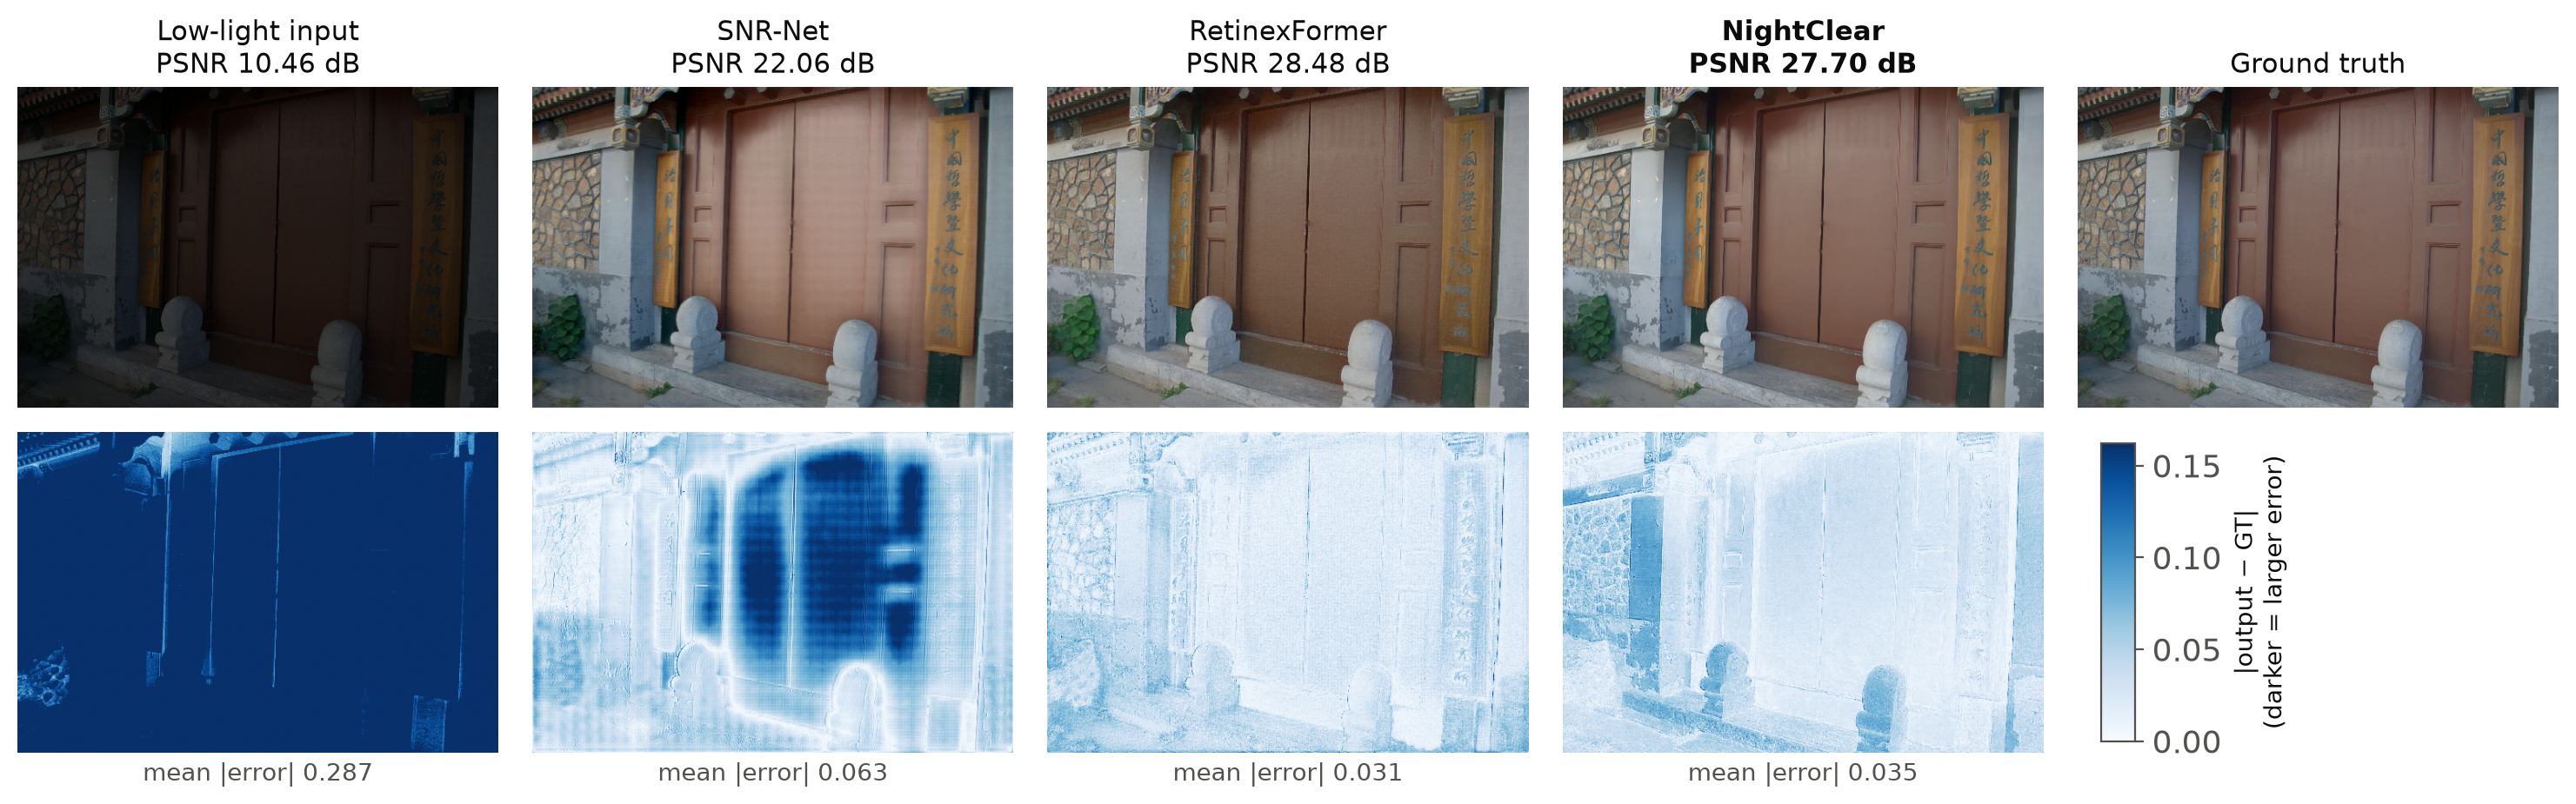
\includegraphics[width=\textwidth, height=0.46\textheight, keepaspectratio]{results/error_maps.png}
    \end{center}
    \footnotesize
    \begin{itemize}
        \item On this image Retinexformer (28.48\,dB) beats NightClear (27.70\,dB): NightClear's errors sit on the \textbf{textured stone wall and dark shadows} (tone shift).
        \item SNR-Net leaves blotchy artefacts on the large flat door.
        \item Takeaway: what remains is mostly \textbf{tone error in dark, textured regions}, consistent with the EDA (very dark pixels carry little signal).
    \end{itemize}
\end{frame}
